%tex_origin: ppt.tex
\subsection{Idea}
\begin{frame}
	\frametitle{Aplicación}
	\begin{itemize}
	\item
		Dos aplicaciones conectadas por sockets, una para el cliente y otra
		para el servidor.
	\item
		El servidor es capaz de aplicar dual-stack, es decir, procesa los
		paquetes sin importar si vienen en IPv4 o IPv6.
	\item
		El cliente es capaz de enviar paquetes de ambos protocolos.
	\item
		Se pueden obtener estadísticas de las operaciones efectuadas (tiempos,
		tazas de perdida, entre otros).
	\end{itemize}
\end{frame}

\begin{frame}
	\frametitle{Aplicación}
	\begin{figure}
		\centering
		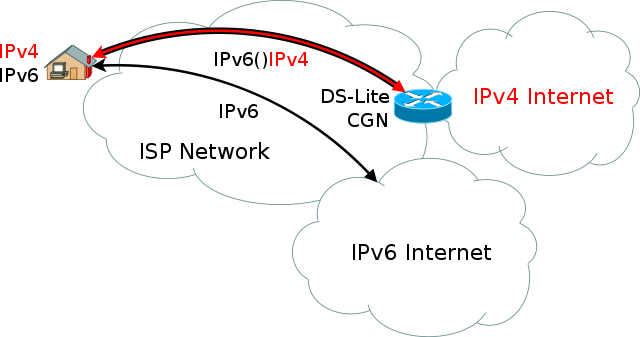
\includegraphics[width=300px]{img/dualstack.png}
	\end{figure}
\end{frame}
